\chapter{Reconstruction of Physics Object}\label{chap:obj}
\vspace{3cm}
To allow the use of all the information enclosed in a bunch crossing, the collection
of all ATLAS detector signals needs to be translated in more user friendly object, 
the reconstruction of the event is carryed out by the ATLAS event reconstruction 
software framework ATHENA~\cite{Athena}. 

Physical particle like electron, muons, hadronic jets, ecc, are all described by means 
of off line software reconstructed object. In section~\ref{} the electron reconstuction 
algorithm is briefly described,
for more details on reconstructed object and their performance see~\cite{AtlasCSCBook}

%In this section the preselection and reconstruction criteria for the
%objects used in this analysis are presented.  For each object and
%selection criteria all corrections that have been applied to data and
%MC are also described.  A summary of the preselection on physics
%objects used in this analysis is reported in Table~\ref{tab:presel}.
\clearpage

\section{Tracks and Vertex Reconstruction}
The reconstruction of charged particles tracks and interaction vertex is based on Inner Detector
information, charged particle bends in the transverse plane due to the magnetic field of the Inner Detector and
this allow to measure their transverse momentum, they can only be reconstructed whithin $|\eta| < 2.5$.
To fully carachterize a track other parameters need to be measured
and those are: the $\phi$ and $\theta$ angles to define its direction, the impact parameter is the 
distance of clostest approach o the track to the beam axis calculated with respect to the origin of coordinate, $d_0$ 
is the impact parameter in the $x-y$ plane,  while $z_0$  is along the $z$ axis.
The transverse impact parameter $d_0$ is the distance of closest approach of the track to the primary vertex
point in the $r-\phi$ projection. The $z$ coordinate of the track at this point of closest approach is referred to $z_0$

\paragraph{Track Reconstruction}
Tracks are reconstructed  by the Inner Detector track reconstruction software~\cite{IDtracking}.
First raw data from the pixel and SCT detectors are transformed in three dimensional space points 
which are called ``hits'', while the  TRT detector information is translated into drift circles. 
Thn, track seeds are formed from a combination of space-points in the three pixel layers and the first SCT layer, these
seeds are then extended throughout the SCT to form track candidates. The tracks candidate are fitted 
using a \emph{Kalman filter} algorothm~\cite{Kalman}, ambiguities in the cluster-to-track association are resolved
and fake tracks are rejected. The selected tracks are then extended to the TRT and finally refitted with the full information of all three
detectors. To help improve tracking efficiency for secondary tracks coming from photon conversion or decays of long-lived 
particles (like kaons), a complementary algorithm searches foir unused track segments in the TRT, which will be then extended
towards the SCT and the pixel in a very similar way as described for the default algorithm.
All tracks found with $\pt > 100$ MeV are written to the database.

%Next, these candidates are
%fitted, “outlier” clusters are removed, ambiguities in the cluster-to-track association are resolved,
%and fake tracks are rejected. 
%
%Silicon pixel, stripes ecc.. responds to te passage of charged particle with a signal,
%those signal are interpreted on a boolean bases and are called ``hits'', 
%The inner detector track reconstruction software [5] follows a modular and flexible software design,
%%which includes features covering the requirements of both the inner detector and muon spectrometer [2]
%%reconstruction. These features comprise a common event data model [6] and detector description [7],
%%which allow for standardised interfaces to all reconstruction tools, such as track extrapolation, track fitting
%%including material corrections and vertex fitting. The extrapolation package combines propagation
%%tools with an accurate and optimised description of the active and passive material of the full detector [8]
%%to allow for material corrections in the reconstruction process. The suite of track-fitting tools includes
%%global-c2 and Kalman-filter techniques, and also more specialised fitters such as dynamic noise adjustment
%%(DNA) [9], Gaussian-sum filters (GSF) [10] and deterministic annealing filters [11]. Optimisation
%%of these tools continues and their performance will need to be evaluated on real data. The tools intended
%%to cope with electron bremsstrahlung (DNA and GSF – see Section 5.1) will be run after the track reconstruction,
%%as part of the electron-photon identification. Other common tracking tools are provided,
%%including those to apply calibration corrections at later stages of the pattern recognition, to correct for
%%module deformations or to resolve hit-association ambiguities.
%Track reconstruction in the inner detector is logically sub-divided into three stages:
%1. A pre-processing stage, in which the raw data from the pixel and SCT detectors are converted
%into clusters and the TRT raw timing information is translated into calibrated drift circles. The
%SCT clusters are transformed into space-points, using a combination of the cluster information
%from opposite sides of a SCT module.
%2. A track-finding stage, in which different tracking strategies [5, 12], optimised to cover different
%applications, are implemented. (The results of studies of the various algorithms are reported else-
%where [13].) 
%
%The default tracking exploits the high granularity of the pixel and SCT detectors to
%find prompt tracks originating from the vicinity of the interaction region. First, track seeds are
%formed from a combination of space-points in the three pixel layers and the first SCT layer. These
%seeds are then extended throughout the SCT to form track candidates. Next, these candidates are
%fitted, “outlier” clusters are removed, ambiguities in the cluster-to-track association are resolved,
%and fake tracks are rejected. This is achieved by applying quality cuts. For example, a cut is made
%on the number of associated clusters, with explicit limits set on the number of clusters shared between
%several tracks and the number of holes per track (a hole is defined as a silicon sensor crossed
%by a track without generating any associated cluster). The selected tracks are then extended into
%the TRT to associate drift-circle information in a road around the extrapolation and to resolve the
%left-right ambiguities. Finally, the extended tracks are refitted with the full information of all three
%detectors. The quality of the refitted tracks is compared to the silicon-only track candidates and
%hits on track extensions resulting in bad fits are labelled as outliers (they are kept as part of the
%track but are not included in the fit).
%A complementary track-finding strategy, called back-tracking, searches for unused track segments
%in the TRT. Such segments are extended into the SCT and pixel detectors to improve the tracking
%efficiency for secondary tracks from conversions or decays of long-lived particles.
%3. A post-processing stage, in which a dedicated vertex finder is used to reconstruct primary vertices.
%This is followed by algorithms dedicated to the reconstruction of photon conversions and of
%secondary vertices.

\paragraph{Vertex Reconstruction}
The vertex recostruction algorithm and its performance are described in full detail in~\cite{AtlasCSCBook,VertexPerf} and
only briefly summarized here.
%say good tracks
The vertex finding is perfomed as follows:  a set of well reconstructed tracks are selected,
a vertex is seeded according to the global maximum of the selected tracks $z$ coordinate distribution, the tracks $z$ coordinate 
is computed with respect the expected averange collision point. 
An adaptive vertex fitting algorithm~\cite{Vertex} determines the vertex position taking as input the vertex seed position and the 
tracks around it. Tracks that are incompatible with the found vertex by more than seven standard deviation
are used to seed the next vertex. The iteration continues untill no tracks are left or no additional vertex can be found.
The procedure depends  on the expected position of the averange interaction point, which is monitored 
during LHC data taking and is computed every few minutes with the method described in~\cite{beamspot}.

The vertex with the larger sum of tracks $\pt$ associated is identified as the \emph{primary vertex} (PV), 
i.e. the interaction point related to the hard scattering of the event. All the other vertices are assumed to result from
minimum bias interaction and are called \emph{pile-up} vertices.
In data recorded during 2012, an averange of 21 multiple interaction are occurred per bunch crossing,
such a high vertex multiplicity strongly affects the ambient energy density in the event, 
a correct pile-up description is then crucial for MC simulation. The ATLAS MC production assures that events 
are simulated with various pile-up conditions, simulated events are then weighted according to the averange interaction
per bunch crossing recorded in data.


\section{Jets Reconstruction and Energy Calibration}
Jets are reconstructed in ATLAS by means of the FastJet package~\cite{fastjet}, 
which provides a broad range of jet finding algorithms and analysis tools. 
In the following jet reconstruction methods relevant for the
analysis presented in this theses are brifly described, for more detail see~\cite{AtlasCSCBook}.

In general, jets may be reconstructed out of any set of four vector objects, 
however in ATLAS, the most important detectors for jet reconstruction are the ATLAS calorimeters.
Calorimeter cells are grouped togheter by a clustering algorithm forming what are called \emph{topological clusters}~\cite{TopoClusterAlgo},
those are three-dimensional cluster representing the energy deposition of the shower.
the clustering starts with seed cells with a signal-to-noise ratio greather that a certain threshold, 
all nearby cells are grouped to the seed cells if they passes a second, lower, signal-to-noise ratio treshould.

Topological clusters are then fed to an \emph{anti-$k_t$} algorithm~\cite{antikt}. The algorithm defines a metric
to assess distances between the clusters $i$ and $j$, the metric is defined as follows:
\begin{align}
d_{ij} &= \text{min}(\frac{1}{k_{t,i}^2}, \frac{1}{k_{t,j}^2}) \cdot \frac{\Delta R_{ij}^2}{R^2}  \\
d_i   &= \frac{1}{k_{t,i}^2} 
\end{align}
where $k_{t,i}$ is the $\pt$ of the cluster $i$ and $\Delta R_{ij}^2 = \sqrt{\Delta\phi_{ij}^2 + \Delta\eta_{ij}^2}$, for
this analysis $R=0.4$ is chosen.
If the distance between two cluster $d_{ij}$ is smaller that $d_i$ the clusters are grouped togheter and their four momentum
summed, otherwise their are kept as single entity. The clustering procedure is iterated until is not possible to merge object
anymore. The metric is designed in a way that high $\pt$ jet will accumulate the soft activity surrounding them leading to conical
jet shapes. 

Given the high pile-up environment of LHC  is important to distinguish jets coming from the hard scattering process and those
related to pile-up interaction, for this purpose a techique, called \emph{jet vertex fraction} (JVF), is implemented in the 
ATLAS jet reconstruction software.
The JVF relies on Inner Detector informations, it is defined as the $\pt$ weighted fraction of tracks pointing
to to the primary vertex associated to the jet:
\begin{equation}
\text{JVF} = \frac{\sum\limits_{PV-tracks}\pt}{\sum\limits_{tracks}\pt}
\end{equation} 
the jet vertex fraction  is only available within Inner Detector coverage $|\eta| < 2.5$,
while calorimeter jet reconstruction is possible up to $|\eta| < 4.5$.

\paragraph{Calorimeter Jet Energy Calibration}
The ATLAS calorimeters were calibrated using test beam electrons~\cite{EMcalibration}, however  the response
to electromagnetic shower  is different from the one to hadronic shower, a dedicated jet energy scale
(JES) calibration is then performed by means of MC simulation~\cite{jesinsitu}: 
jet energy is corrected to correspond, as a mean value, to the simulated energy 
of the hadronizing parton origin of the jet. The direction of the jet is also corrected to constraint it to point
to the primary vertex instead to the center of the ATLAS detector. A set of corrections are then evaluated to take into account
effect of pile-up~\cite{jespileup, jesarea}. Jet resolution is also corrected in MC to better describe the data~\cite{jer}. 
Finally, several jet energy scale correction are applied for a better agreement between 
data and simulation, those corrections are evaluated based on 2011 ATLAS data compared to MC simulation and 
exploits several techniques, JES systematic uncertainty due not perfect MC modeling are also evaluated,
a full description of JES "in-situ" methodology corrections and related systematics uncertainties are 
described in~\cite{jesinsitu, JES}. %all the correction are combined toghether obtaining the final JES


\section{Jet b-Tagging}
Typical decay lenght of b-hadron at ATLAS is of the order of few millimeter, exploiting the high precision of the
Inner Detector tracker is possible to identify jet originatig from b-quarks with respect to other flavors, 
those jets are called \emph{b-jets} and the identification technique used \emph{b-tagging}.

Several algorithm has been developed in ATLAS for jet b-tagging, the relevant b-tagging algorithm
to this thesis are briefly described in what follows, for more detailed description see~\cite{AtlasCSCBook}.
The first step of jet b-tagging is to associate tracks to jets based on a $\Delta R$ cone matching, those tracks 
should satisfy strict selection criteria aimed to assure good quality 
and to reject tracks likely to come from strange hadron decays or photon conversion. 
For the discrimination between b-jet or light-jet (and in some cases also c-jet) 
algorithms uses the MC prediction of the distribution of some discriminating variable 
for the two hypotesis.
Given the relatively high mass of b-hadrons, the tracks
associated with b-jet will have spreaded impact parameters, this feature is used by the IP3D b-jet tagging 
algorithm, in which is implemented a discriminatig variable based on the sum of the impact parameter significances of all the tracks
associated to the jet. An alternative approach, used by the $SV1$ algorithm, is instead  to searches for inclusive 
secondary vertex formed by the decay products of the b-hadron,  the search includes also 
the subsequent charm hadron decays. Another algorithm, called JetFitter~\cite{jetfitter}, uses instead the direction of the jet
to fully reconstruct the decay chain of b-hadron, the assuption made is that the decayed particles will lie along the
jet axis. Finally, the three algorithm just described are combined togheter using an
artificial neural network to maximize the discriminating power, the output of this neural network is referred
as $MV1$ and is used in the search presented in this thesis. 

\begin{figure}[tp]
     \begin{center}

            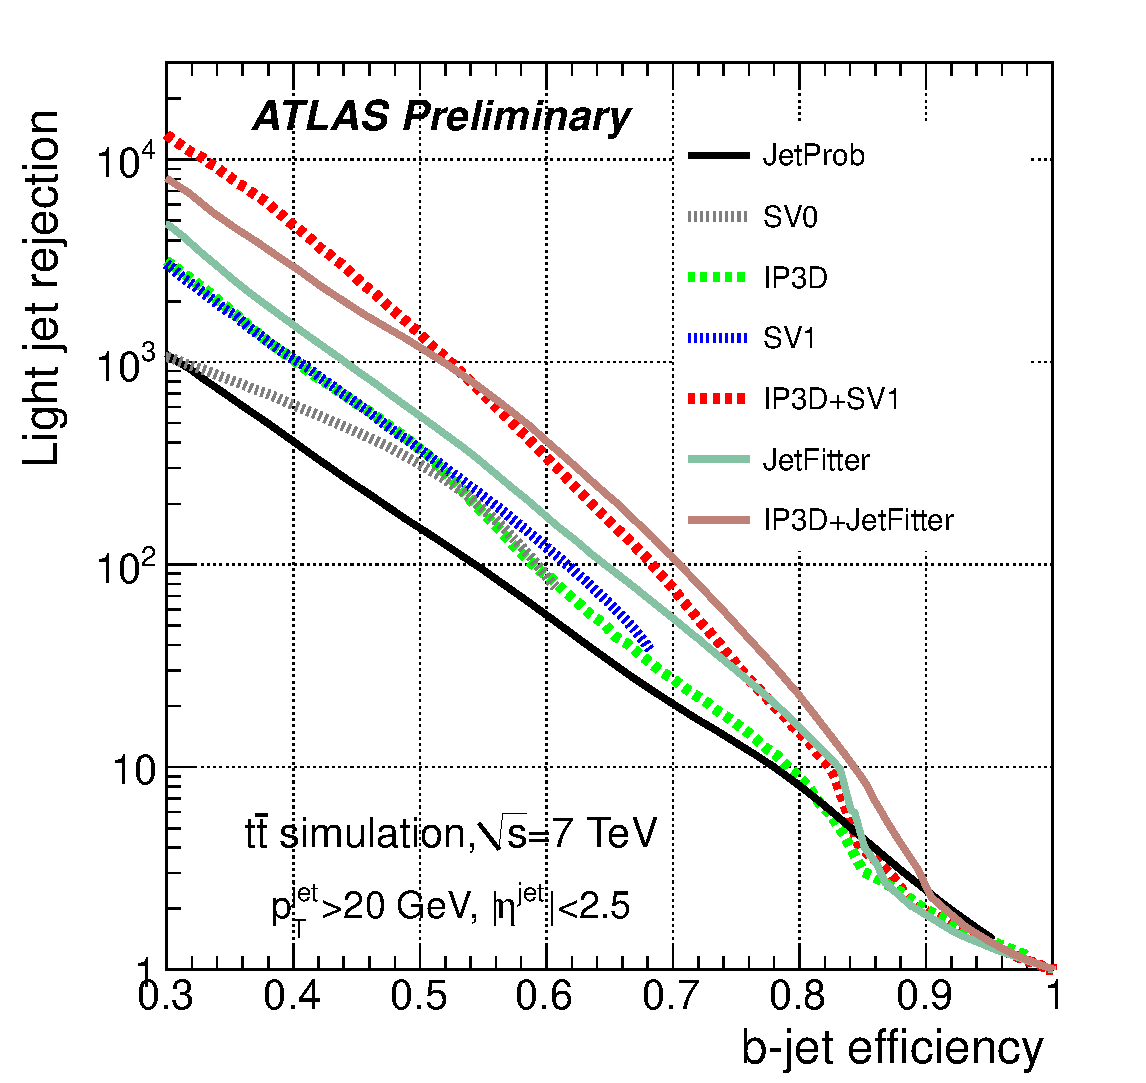
\includegraphics[width=0.6\textwidth]{figure/obj/btag_perf.pdf}

    \end{center}
    \caption{Light-jet rejection as a function of the b-jet tagging efficiency for different tagging algorithms~\cite{btagPerf}.
	    Rejection here is defined as the inverse of mistagging rate, and the distributions are referred to a 
		$\ttbar$ sample.}
   \label{fig:beff}
\end{figure}

The perfomance of the mentioned algorithms are evaluated in data  and compared to simulation in~\cite{btagPerf}.
B-hadron tagging efficiency and mistagging rate are the most common feature that describes the performance of a
b-tagging algorithm, Figure~\ref{fig:beff} shows the b-tagging efficiency as a fuction of the inverse of the mistagging rate
for different b-tagging algorithm, the tagging efficiency $\epsilon_b^{\ttbar}$ is usually referred to b-hadron in $\ttbar$ events
and totally specify a b-tagging selection point.
Correction due to non perfect modeling of b-tagging performance are evaluated by means of several methods
for 2012 data in~\cite{BtaggingScaleFactors, BtaggingScaleFactorsNew} and used as event weights in MC simulation.



\section{Electrons Reconstruction} \label{sec:elec}
Electron are reconstructed combining calorimeter and Inner Detector information,
an electron dedicated reconstruction algorithm is presented in~\cite{electronAlgo} is based on clusters reconstructed in the electromagnetic
calorimeter, which then are associated to tracks of charged particles reconstructed in the Inner Detector.


This analysis uses electrons found by the standard electron
identification algorithms ~\cite{AtlasCSCBook} that pass the {\tt Medium++}
criteria. A preselection is applied to the electrons to ensure that
the electron cluster has a transverse energy of $E_T > 15\GeV$, is
within the pseudorapidity range $|\eta|<2.47$, but is outside of the region
$1.37<|\eta|<1.52$. The first requirement ensures that the selected
electrons are within a range of $E_T$ where the electron reconstruction
and trigger efficiencies are well understood. The further requirements
ensure that the electron is reconstructed within the acceptance of
the ATLAS tracking, but outside of the transition region between the
barrel and end-cap calorimeters. 
In addition, the author is required to be either one or three, to ensure that the electron was 
reconstructed with either the standard electron algorithm or both the
standard and soft electron algorithms, respectively.
Finally, to ensure that the electron is not reconstructed within a region of the
calorimeter with readout problems, dead or non-nominal high voltage
conditions or suffering from high noise, the electron is rejected if
the cluster $\eta$ and $\phi$ position match a flagged region in the
Object Quality maps (OQ maps) provided by the egamma
performance group~\cite{EGammaRecomendations}.

For the electrons used in this analysis, the four-vector of the
particle is defined using the energy of the electron calorimeter
cluster and the direction of the electron track. Selections that
involve the electron position in the calorimeter, in this analysis the
$\eta$ and the OQ map selections, are however made using a four-vector built
entirely from the electron cluster properties. Both the energy scale
and resolution of the electrons used in this analysis are corrected,
following the recommendations of the EGamma performance group, by
using the {\tt egammaAnalysiUtils}
package\cite{EGammaRecomendations}. Energy scale corrections are
applied to electrons in data, whereas an additional smearing is
applied to the electron energy in MC.

In addition to the preselection defined above, isolation criteria are
defined to select electrons with little or no activity around
them. The calorimetric isolation, \etcone, is calculated as the sum of
the transverse energy of the additional topological clusters in the
electromagnetic and hadronic calorimeters in a cone of $\Delta R <
0.2$ around an electron\footnote{The $\Delta R$ variable is defined by
$\Delta R=\sqrt{(\Delta\eta)^2+(\Delta\phi)^2}$, where $\Delta \eta$
and $\Delta \phi$ correspond to the difference between
the pseudorapidities and azimuthal angles of the objects considered, respectively.}. 
The summed transverse energy is corrected, as a function of the
number of primary vertices in the event, to reduce the dependence on
pileup. In addition, the track isolation, \ptcone, is defined as the
scalar sum of the $\pt$ of all additional tracks with $\pt>1\GeV$ in a
cone of radius $\Delta R<0.4$ around an electron. In this analysis, an
electron with $\etcone/\pt<0.08$ and $\ptcone/\pt<0.06$ is considered isolated.


\subsection{Muons}
\label{sec:presel:muon}

Muons reconstructed by the STACO algorithm \cite{AtlasCSCBook} are
used in this analysis - those passing the STACO Loose quality criteria
are considered at the preselection stage, whereas the more stringent
STACO Combined quality criteria are required for the final muon
selection. Muons with a transverse momentum $\pt > 10\GeV$ and
within the pseudorapidity range $|\eta| < 2.5$ are selected. The
difference between the $z$ position of the muon track extrapolated to
the beam line and the primary vertex $z$ position must be less than 10
mm. 

Further quality criteria, as recomended by the Muon Combined Performance Group,
 are placed on the Inner Detector track of
the muon candidate to ensure that it is well reconstructed and to
reduce the fake rate due to decays of hadrons in flight. These
requirements ensure that multiple hits are found on the track in the
various layers of the ID, but take into account that dead or
uninstrumented regions may be crossed by the muon. Firstly, if the
muon passes through a section of the b layer of the Pixel detector
that is instrumented and not suffering from detector problems, there
should be one or more b layer hits on the track. The sum of the number
of hits on the track in the Pixel detector and the number of crossed
dead Pixel detector layers should be at least one. The sum of the
number of hits within the SCT detector and the number of dead SCT
modules crossed should be five or greater. The total number of crossed
dead Pixel detector and SCT detector layers should be less than three.
When within the angular region $|\eta|<1.9$, the sum of the TRT hits
and outliers on the track must be greater than five and the ratio of
TRT outlier hits to the total number of TRT hits must be less than
0.9. When the muon track is in the region $|\eta|\ge1.9$, the ratio of
TRT outlier hits to the total number of TRT hits must be less than 0.9
only if the sum of the TRT hits and outliers on the track is be
greater than five.

The momentum scale and resolution of the muons in this analysis are
corrected in MC following the recommendations of the Muon Combined
Performance group. The momentum corrections were measured by comparing
the di-muon mass peak position and resolution between data and MC at
the Z resonance. Smearings are applied in a coherent manner to
the ID, MS extrapolated and combined momenta of the transverse
momentum of the muon. In addition, a scale correction is applied to
the combined momentum momentum.

As for the electrons used in this analysis, both calorimeteric and
track based isolation are used to require little or no activity around a muon
in addition to the preselection above. The muon \etcone and \ptcone
variables are defined as for the electron case and are calculated
in cones of $\Delta R<0.2$ and $\Delta R<0.4$ around the muon, respectively. 
Once more \etcone is corrected as a function of the number of primary vertices in the
event, to reduce the dependence on pileup. In this analysis, a muon with
$\etcone/\pt<0.04$ and $\ptcone/\pt<0.06$ is considered isolated.



\subsection{b-Tagging}
\label{sec:presel:btag}

The tagging of jets due to the hadronisation of b-quarks is performed
using the MV1 b-tagging algorithm \cite{mv1}. This neural network based
algorithm uses the output weights of the JetFitter+IP3D, IP3D and
SV1 b-taggers as inputs. The working point that gives a nominal
b-tagging efficiency of 70\% on \ttbar samples is used.

\subsection{Taus}
\label{sec:presel:tau}

Hadronically decaying tau candidates are reconstructed using clusters
in both the electromagnetic and hadronic calorimeters. A preselection
is applied to the candidates that requires the reconstructed $\tau$
candidates to have a transverse momentum of $\pt>20 \GeV$ and to have
a reconstructed pseudorapidity of $|\eta| < 2.5$. Furthermore, it is
required that the candidates have either one or three tracks within a
cone of $\Delta R < 0.2$ associated to them and have a charge of $\pm
1$. Finally, the preselected tau candidates should pass the BDT-Medium
multivariant tau identification selection as well as the dedicated
electron and muon vetoes for hadronically decaying tau candidates.


\subsection{Overlap Removal}
\label{sec:presel:olr}

After the preselection of the physics objects needed for this
analysis, an overlap removal between the different objects is then
applied to avoid double-counting.  The distance between two objects in
rapidity $\Delta\eta$ and polar angle $\Delta\phi$ is defined as
$\Delta R=\sqrt{(\Delta\eta)^2+(\Delta\phi)^2}$. Overlap removal is
then applied in the following order:

\begin{itemize}
\item preselected electrons are removed if they overlap with a preselected muon  within $\Delta R < 0.2$,
\item preselected taus are removed if they overlap with a preselected muon or electron within $\Delta R < 0.2$,
\item preselected jets are removed  if they overlap with a preselected
  muon, electron or tau within \linebreak $\Delta R<0.2$.
\end{itemize}

\subsection{Missing Transverse Energy}
\label{sec:presel:met}

The missing transverse energy, \met, is calculated using the
RefFinal method, which takes the energy
deposited in the calorimeter, the muons reconstructed in the muon
spectrometer and tracks reconstructed in the inner detector as inputs. 
For this, the energy deposits are calibrated based
upon the high-$pt$~ physics object they are associated to, with an order
of preference of electrons, photons, hadronically decaying taus, jets
and finally muons. Any unassociated energy deposits are combined into
the so-called ``soft-term''. To reduce the effect of pileup on the
\met calculation, corrections are applied to both the jets in an event
and to the soft-term. Firstly, any jet with a pseudorapidity of $|\eta|<2.4$
that enters the \met calculation is weighted by it's JVF. Similarly,
the soft-term is weighted by the soft-term-vertex-fraction (STVF) of
the event - the ratio given by
\begin{equation}
STVF = \frac{\sum_{track, PV}\pt}{\sum_{track}\pt}
\end{equation}
where $\sum_{track, PV}\pt$ is the sum of the transverse momentum of
all tracks in the event associated to the primary vertex, but unmatched to physics
objects, and $\sum_{track}\pt$ is the sum of
the transverse momentum of all tracks in the event unmatched to
physics objects. Any calibration applied
to the energy or direction of the physics objects in the final
analysis is also propagated to the \met.


\subsection{Vertices} 
\label{sec:presel:vertices}
In this analysis vertices are selected that have a minimum of three
associated tracks: this helps to ensure that the selected vertices
come from beam-beam interactions rather than, for instance, cosmic
muons.

\subsection{Event Cleaning}
\label{sec:presel:celaning}

In addition to the data quality requirements described in section
\ref{sec:samples:dq}, further selections are applied to veto events
where bad jets are identified as arising from detector effects
(coherent noise in the EM and Tile calorimeters or spikes in the HEC
calorimeter), cosmics or beam based background. To reject events, the
recommendations of the JetEtMiss performance group \cite{TWIKI_JETMET}
are followed: Events are rejected if at least one AntiKt4LCTopo jet
with $p_T>20\GeV$, that passes the overlap removal with electrons,
muons and taus described in section \ref{sec:presel:olr}, fails the {\tt
BadLooseMinus} selection or points towards the hot Tile Calorimeter
cells identified in data taking periods B1 and B2 \cite{hottile}.

\begin{table}
  \begin{center}
    \begin{tabular}{cc}
      \hline \hline
      Physics Object & Preselection \\
      \hline
      Electrons & $\pt>15 \GeV$ \\
      & $|\eta|<1.37$ or $1.52<|\eta|<2.47$ \\
      & {\tt Medium++} \\
      & Author = 1 or 3 \\
      & Pass Object Quality Flag \\
      \hline
      Muons & $\pt>10 \GeV$ \\	
      & $|\eta|<2.5$ \\
      & isLoose STACO muon \\
      & Inner Detector track quality requirements \\
      & Inner Detector track $|z_0^{PV}|<10\mathrm{mm}$ \\
      \hline
      Jets & $\pt>30\GeV$ \\
      & $|\eta|<4.5$ \\
      & $|JVF|>0.5$ for jets with $|\eta|<2.4$ and $\pt<50\GeV$ \\
      \hline
      Jets (taggable) & $\pt>20\GeV$ \\
      & $|\eta|<2.5$ \\
      & $|JVF|>0.5$ for jets with $|\eta|<2.4$ and $\pt<50\GeV$ \\
      \hline
      Taus & $\pt>20 \GeV$ \\	
      & $|\eta| < 2.5$ \\
      & BDT Medium \\
      & $N_{tracks} =~ $1 or 3 \\
      & Author = 1 or 3 \\
      & Muon and Electron Veto \\
      \hline
      \met & RefFinal with STVF correction\\	
      \hline
      Vertices & $N_{tracks} \ge 3$ \\	
      \hline \hline
    \end{tabular}
    \caption{Summary of the preselections used for physics objects in this analysis}
    \label{tab:presel}
  \end{center}
\end{table}


\subsection{Monte Carlo Corrections}
\label{sec:presel:MCCorr}

The MC samples used on this analysis are corrected to account for differences
between the simulation and data in the trigger, lepton reconstruction and
identification and b-tagging efficiencies. Furthermore, the MC is
reweighted so that the vertex multiplicity distribution agrees with
that in the data.

\subsubsection{Trigger Efficiency corrections}
\label{sec:presel:TriggerCorr}

Correction factors are applied to the simulated trigger efficiency for
both the single electron, \linebreak \verb=EF_e24vhi_medium1=, and combined
electron-muon, \verb=EF_e12Tvh_medium1_mu8=, triggers used in this
analysis. The trigger efficiency for the \verb=EF_e24vhi_medium1= has
been measured with respect to offline electrons using a tag and probe
method in \Zee events \cite{TWIKI_EgammaWG_Eff_SF}. Scale factors are derived from the ratio of the
trigger efficiency measured in data and MC, measured as a
function of electron $\pt$ and $\eta$.

For the \verb=EF_e12Tvh_medium1_mu8= trigger, correction factors are
measured separately for the two individual legs of the trigger,
\verb=EF_e12Tvh_medium1= and \verb=EF_mu8= \cite{TriggerEfficiency}. The product of the two
correction factors is then used as the overall scaling factor. The
trigger efficiency for the \verb=EF_e12Tvh_medium1= leg has been
measured with respect to offline electrons using a tag and probe
method for \Zee events in both data and MC. Likewise, the
\verb=EF_mu8= trigger efficiency scale factors are derived using a tag
and probe measurement with \Zmumu events. Oncemore, scale factors are derived
from the ratio of the trigger efficiency measured in data and MC, measured as a
function of electron $\pt$  and $\eta$.

\subsubsection{Lepton Reconstruction Efficiency Corrections}
\label{sec:presel:LepEffCorr}

Further correction factors are applied to the MC samples to account
for differences in the lepton reconstruction and identification
efficiencies between data and simulation. Scale factors for the electron
identification and reconstruction efficiencies are measured separately
using a combination of $\Zee$ and $J/\psi \rightarrow ee$ tag and probe
measurements \cite{EGammaRecomendations}. 
Both sets of scale factors are measured as a function of the electron $E_T$ and $\eta$. 

Similarly, muon reconstruction efficiency scale factors
have been measured, using a \Zmumu tag and probe analysis, 
as a function of the muon $\pt$, $\eta$, $\phi$ and charge \cite{MuonReconstruction}.

\subsubsection{b-tagging Efficiency Corrections}
\label{sec:presel:BTagEffCorr}

Corrections are applied to the b-tagging efficiency and mistag rate in
MC, using a combination of the System8 and likelihood scale
factor measurements \cite{BtaggingScaleFactors}. Separate scale factors are applied, 
as a function of the jet \pt and $\eta$, 
based on the origin of the jet at truth level - ie. depending on if the jet originates from a $b$ quark, a $c$ quark, a $\tau$ lepton 
or a light quark.

\subsubsection{Pileup Reweighting}
\label{sec:presel:PileupCorr}

Differences between the distribution of the average number of
interactions per bunch crossing, $<\mu>$, in MC and data are
corrected by reweighting the MC $<\mu>$ distribution to that in the
full considered dataset. An additional scaling of $1.1 \times <\mu>$
is applied to the MC, which has been shown to improve the description
of the number of primary vertices distribution of the data.

